% Highlight Box
\definecolor{teal}{rgb}{0.99,0.37,0.53}
\newmdenv[innerlinewidth=0.5pt, roundcorner=4pt,linecolor=teal,backgroundcolor=teal,innerleftmargin=6pt,
    innerrightmargin=6pt,innertopmargin=6pt,innerbottommargin=6pt,leftmargin=-9pt,rightmargin=-9pt]{mybox}

Temporal Difference (TD) learning estimates the value function of a Markov Reward Process (MRP) using samples of successive differences. This is done with the Bellman equation:
\begin{center}
    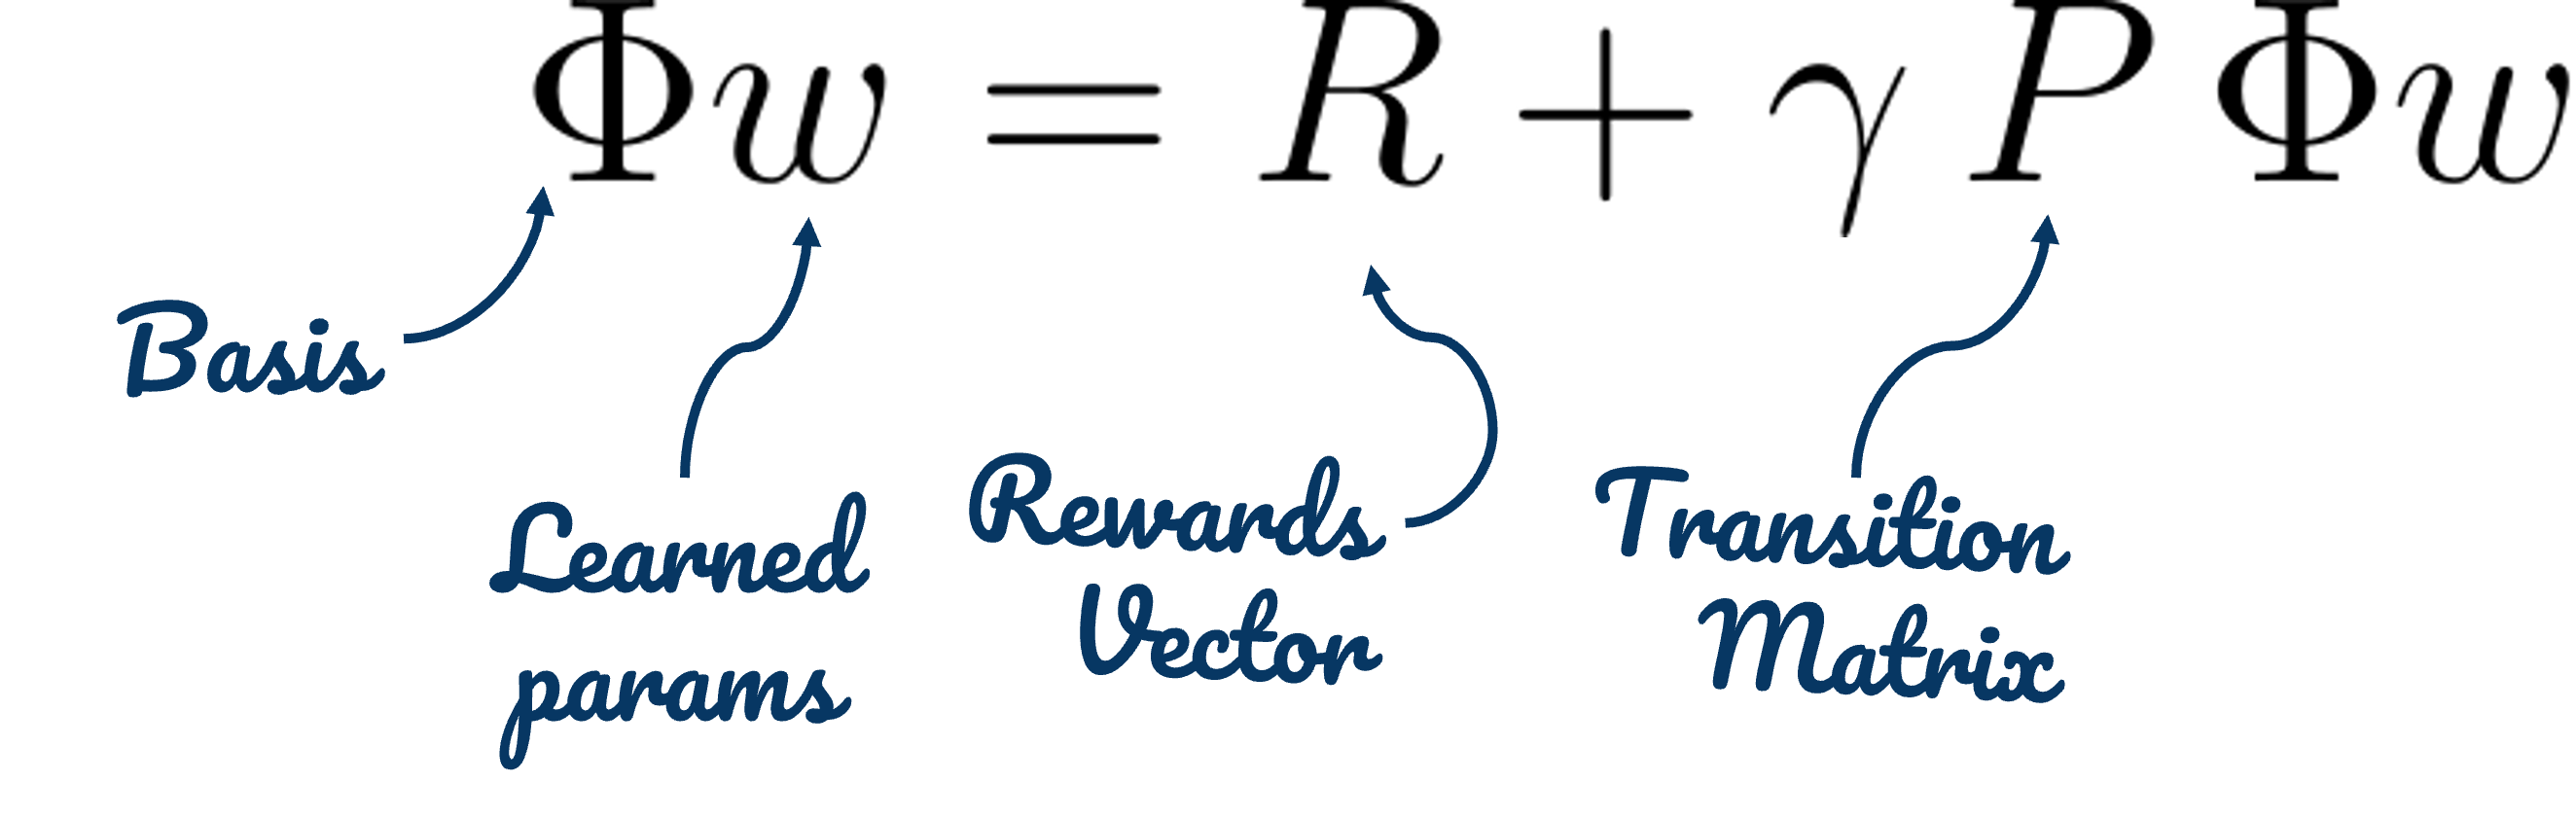
\includegraphics[scale=0.4]{parts/intro/bellman}
\end{center}\vspace{-.1in}
TD may learn arbitrarily bad value functions under \emph{Deadly Triad} conditions:
bootstrapping (learning from your own output),
function approximation, and
off-policy updates.
\vspace{-.11in}
\begin{center}
    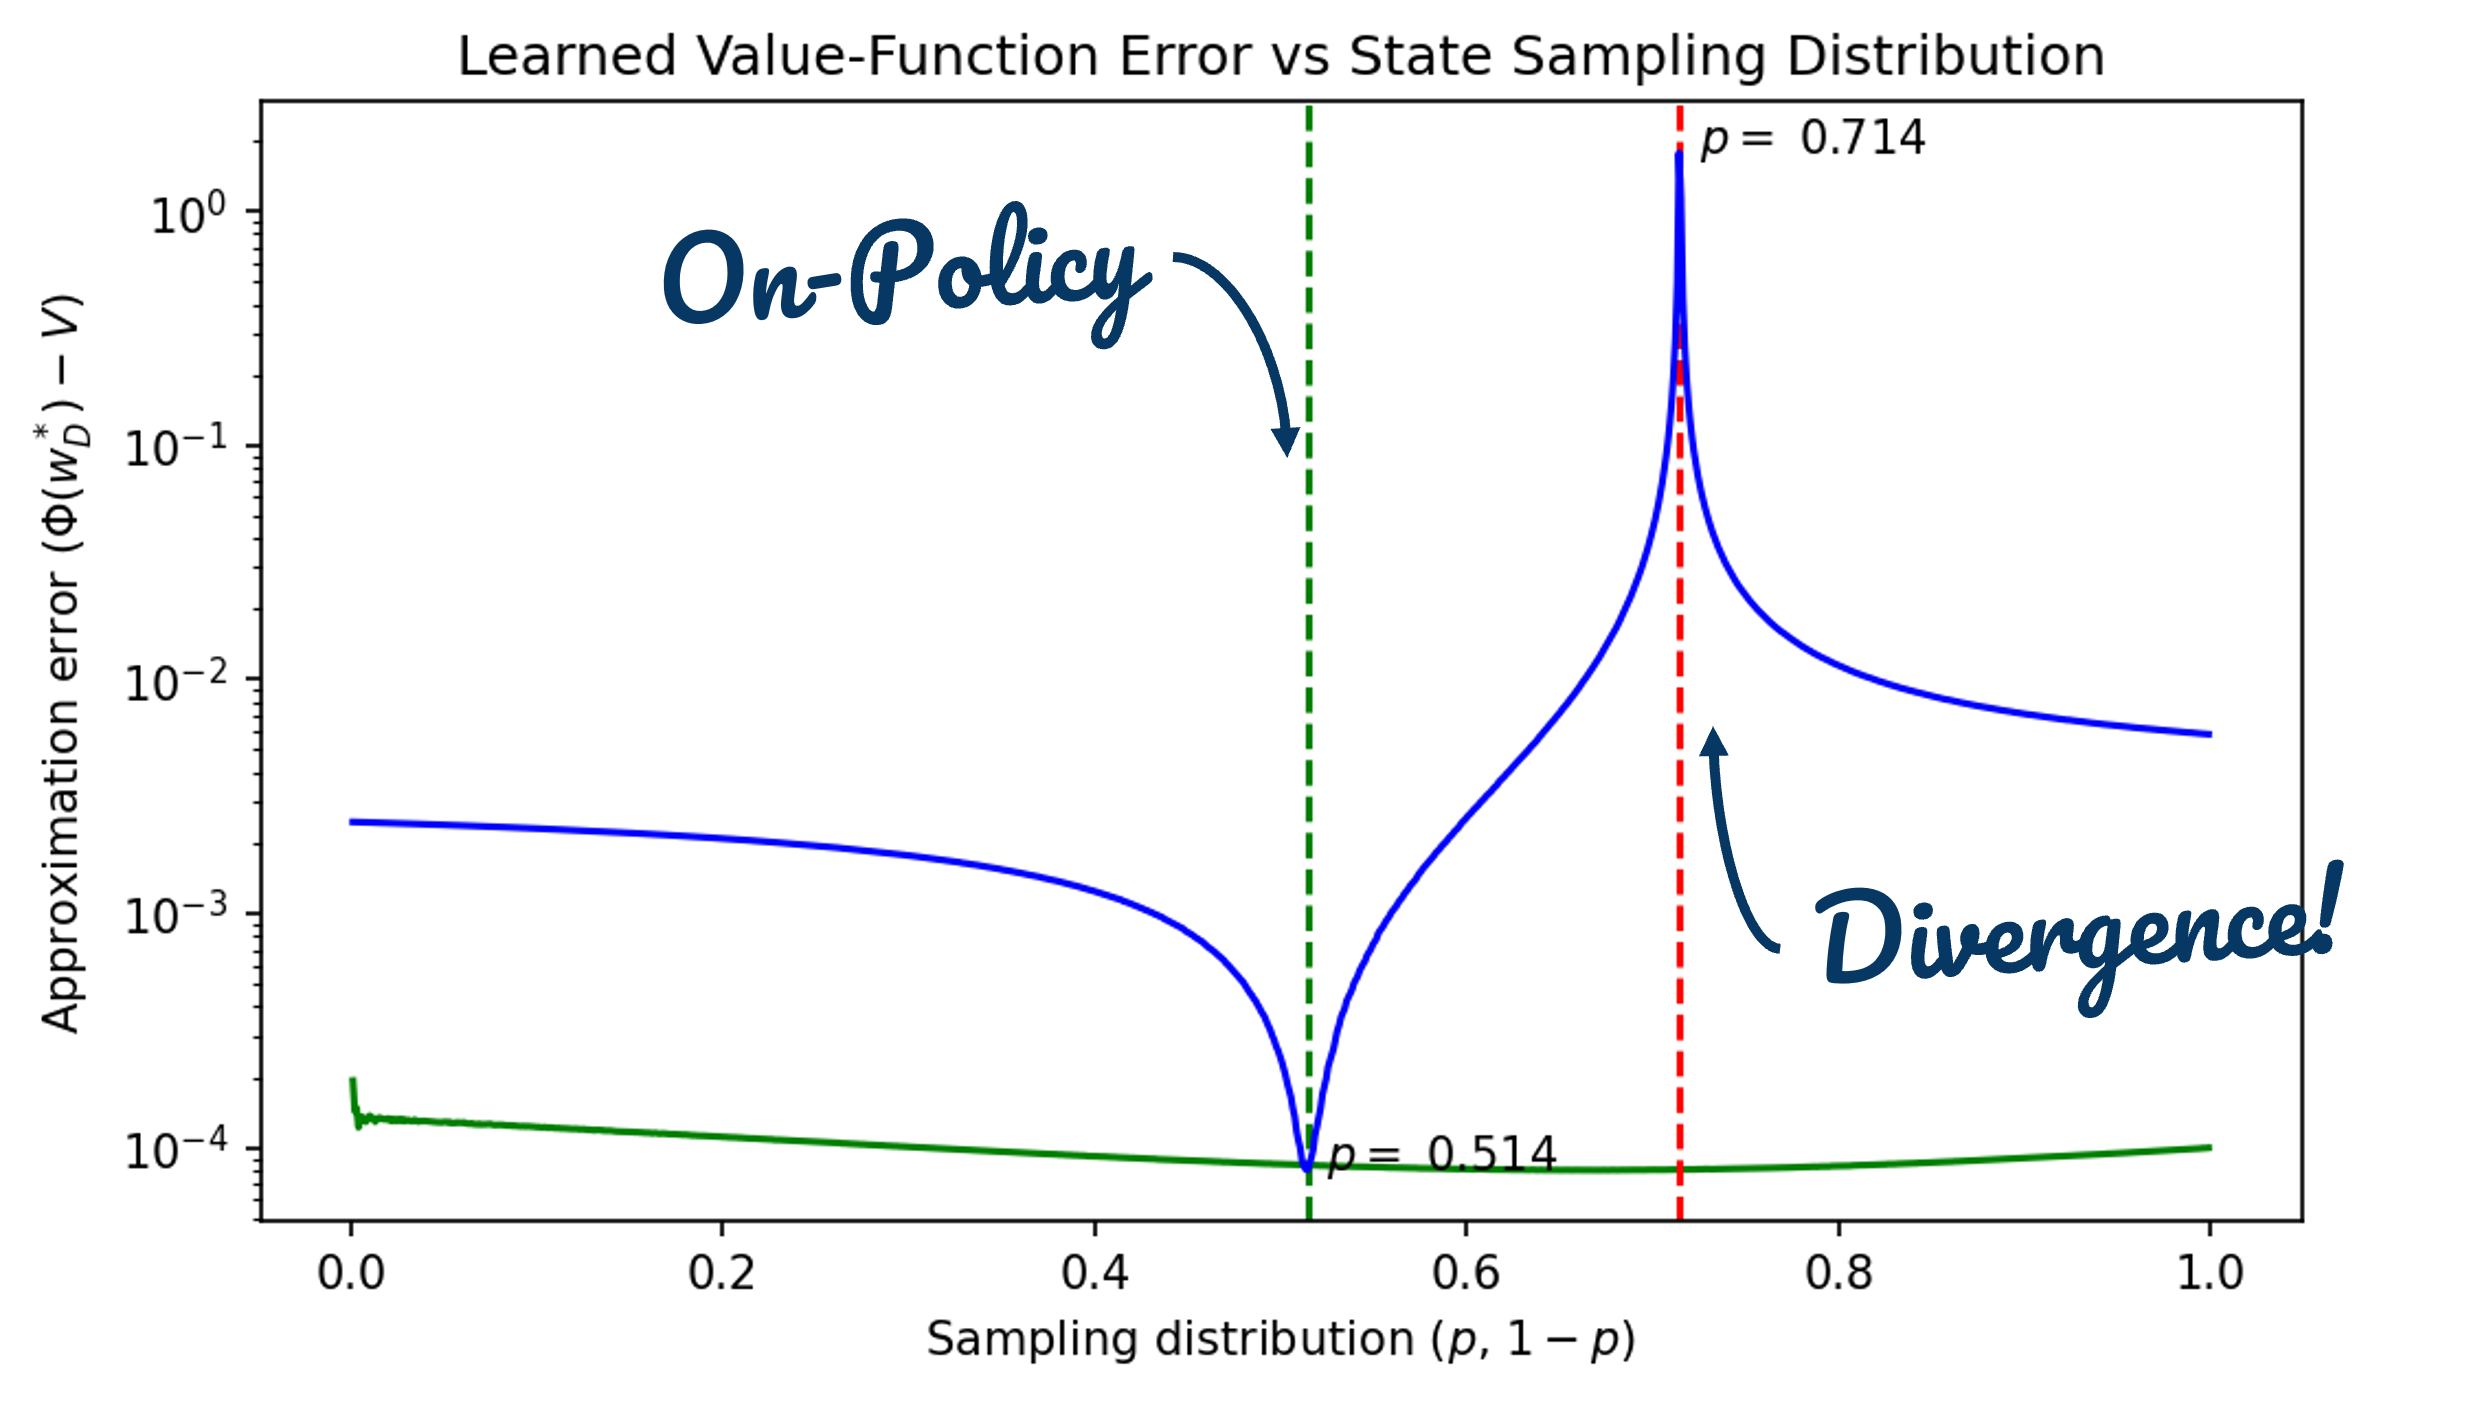
\includegraphics[scale=0.4]{parts/intro/threestatedivergence}
\end{center}\vspace{-.1in}
Regularization is a popular mitigation, and is supposed to work like this:
\begin{center}
    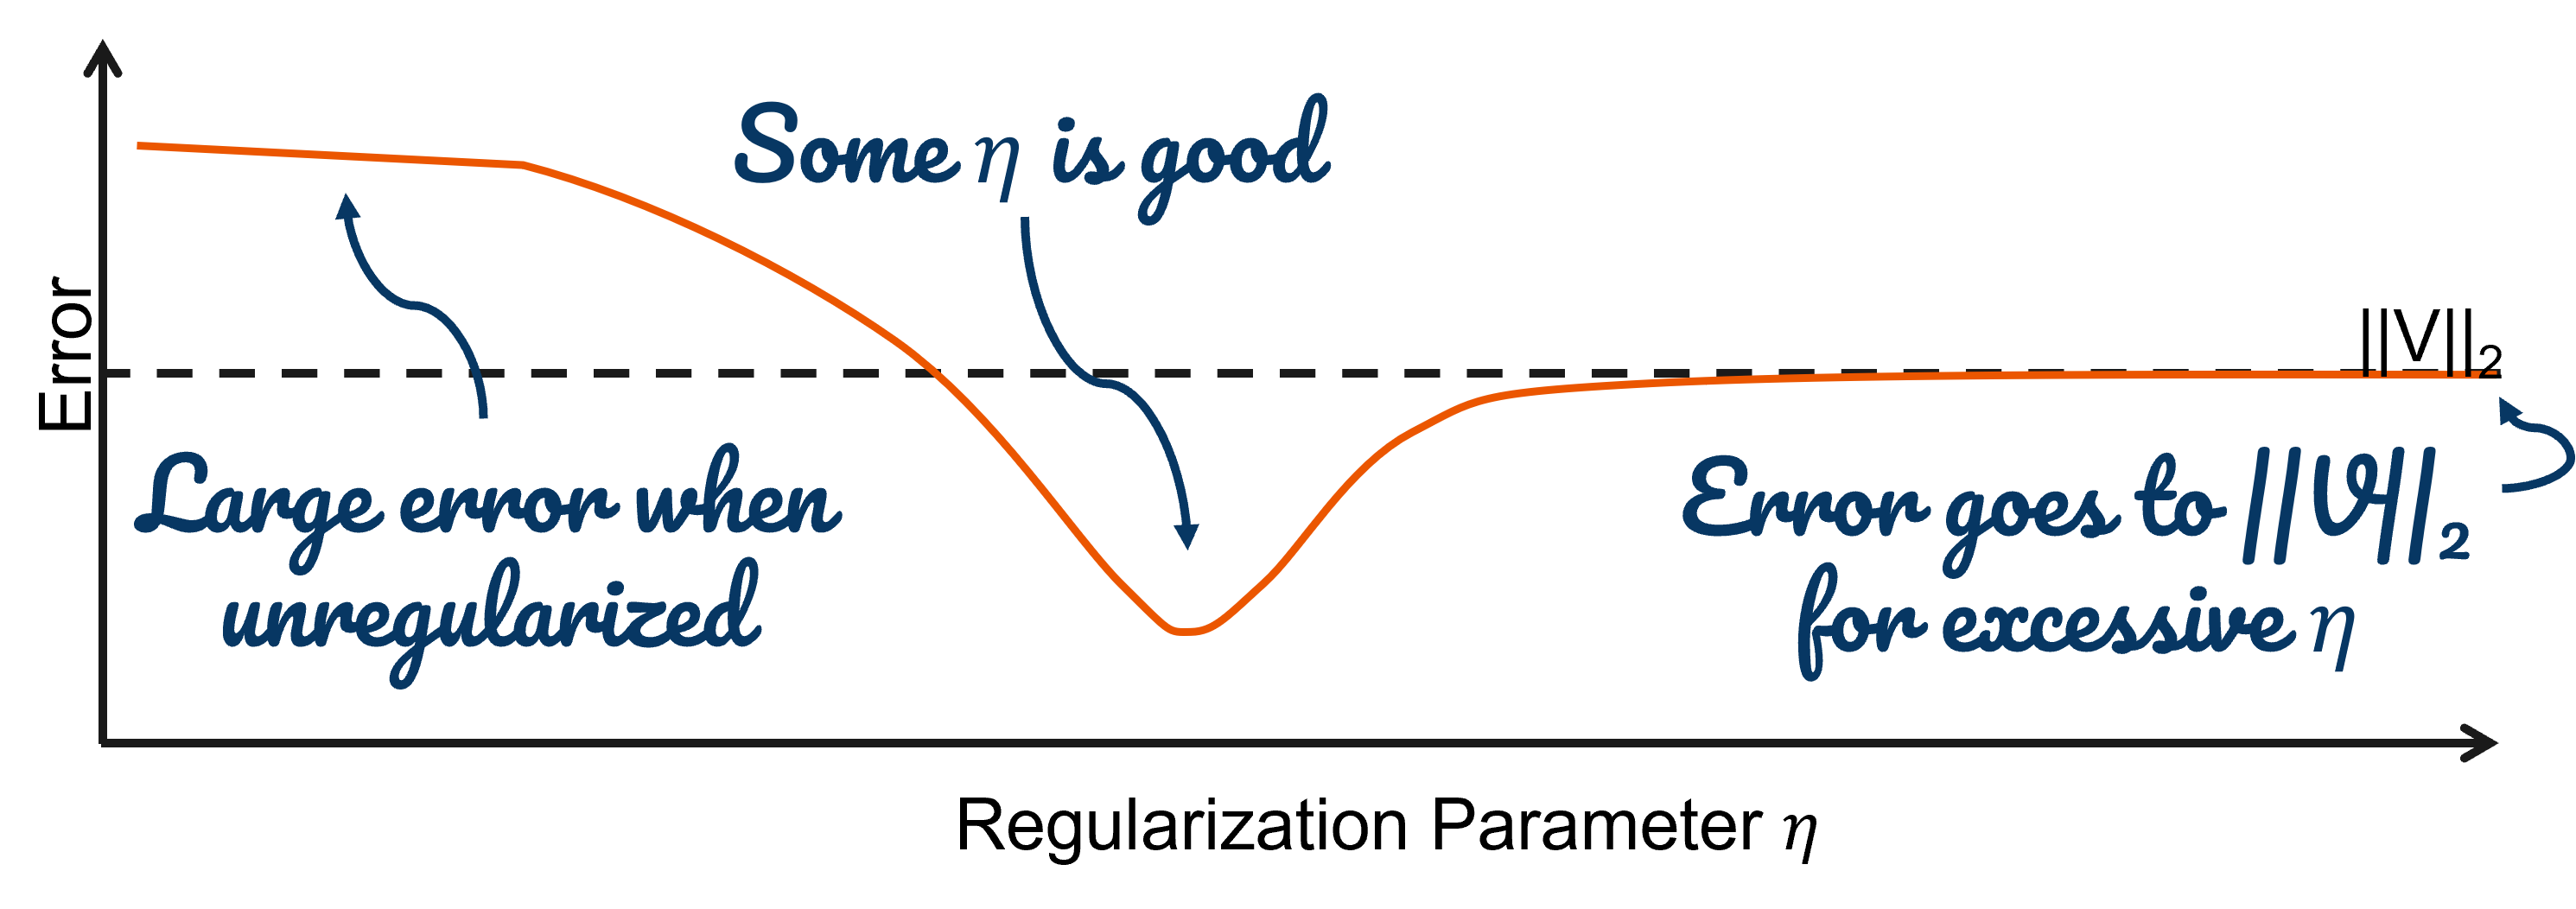
\includegraphics[scale=0.4]{parts/intro/regworks}
\end{center}
\begin{mybox}
    {\headerfont Regularization doesn't always work!}
    \vspace{.5em}
    {\large
        \begin{enumerate}
            \item Models may be \emph{vacuous}.
            \item Regularizing TD is \emph{not monotonic}.
            \item Emphatic models are \emph{not immune}.
        \end{enumerate}
    }
    \vspace{.5em}
\end{mybox}